\apendice{Especificación de Requisitos}

\section{Introducción}

La Especificación de Requisitos Software \textit{(ERS)} es el documento intermediario entre los desarrolladores y los clientes. 
En este se exponen los objetivos respecto al software y los requisitos para conseguir el resultado esperado. \\
En las siguientes secciones se analizarán cada uno de los requisitos necesarios, tanto funcionales como no funcionales, con sus respectivos casos de uso.

\section{Objetivos generales}
Al comienzo del desarrollo del proyecto, se marcaron unos objetivos a cumplir:
\begin{enumerate}
    \item \textbf{Aplicación web:}\\
    Crear una página web funcional que permita realizar el análisis de datos extraídos de Twitter.
    \item \textbf{API de Twitter:}\\
    Conectar con la API de Twitter para la obtención de datos de la red social Twitter.
    \item \textbf{Base de datos:}\\
    Conectarse con una base de datos para almacenar la información extraída de Twitter y más tarde recuperarla para la realización de estadísticas.
    \item \textbf{Patrimonio histórico \textit{BICs}:}\\
    Selección del patrimonio histórico del tramo del camino Francés en Castilla y León de la que se requieren los gráficos estadísticos.
    \item \textbf{Estadísticas temporales:}\\
    Visualizar gráficamente la información almacenada en la base datos.
    \item \textbf{Análisis de sentimientos:}\\
    Calcular un índice de sentimiento (negativo o positivo) de cada tweet. Visualizar los valores medios de sentimiento de los tweets de cada patrimonio.
\end{enumerate}
\section{Catalogo de requisitos}
A continuación se detallarán cada uno de los requisitos, tanto funcionales como no funcionales de la aplicación del proyecto.
\subsection{Requisitos funcionales}
Los requisitos funcionales son cada una de las tareas que satisfacen las necesidades del usuario y que pueden ser detectadas por el mismo. \\
Estas se han desarrollado a lo largo del proyecto hasta cumplir con su funcionalidad.

\begin{itemize}
    \item \textbf{RF1-Visualización de datos estadísticos:} La aplicación debe ser capaz de mostrar los datos estadísticos de los tweets.
    \begin{itemize}
        \item \textbf{RF1.1-Gráfico temporal:} La aplicación debe mostrar un gráfico de los tweets sobre el patrimonio elegido entre un periodo de tiempo.
        \item \textbf{RF1.2-Gráfico porcentual:} La aplicación debe ser capaz de mostrar un gráfico circular del porcentaje de tweets sobre el patrimonio elegido respecto al resto de patrimonios.
        \item \textbf{RF1.3-Gráfico de datos públicos:} La aplicación debe ser capaz de mostrar un gráfico de barras comparando los parámetros públicos de los tweets del BIC elegido entre un periodo de tiempo.
        \item \textbf{RF1.4-Selección de fechas:} El usuario debe poder seleccionar las fechas entre las que requiere las estadísticas patrimoniales.
        \item \textbf{RF1.5-Análisis de sentimientos:} La aplicación debe ser capaz de mostrar gráficamente los valores medios de sentimiento de los tweets de cada patrimonio.
        \item \textbf{RF1.6-Gráfico de estadísticas generales:} La aplicación debe ser capaz de mostrar gráficamente el total de los tweets de todos los BICs.
    \end{itemize}
    \item \textbf{RF2-Mapa de patrimonios:} La aplicación deberá mostrar en un mapa cada uno de los BICs en su localización real.
    \begin{itemize}
        \item \textbf{RF2.1-Mostrar nombre de patrimonio:} El usuario debe poder ver el nombre del BIC al que se refiere cada una de las localizaciones.
        \item \textbf{RF2.2-Selección de BIC:} El usuario debe poder seleccionar un bien de interés cultural en el mapa y realizar estadísticas.
    \end{itemize}
    \item \textbf{RF3-Barra navegadora:} La aplicación debe tener una barra navegadora para redireccionarse a otras páginas de la aplicación.
    \begin{itemize}
        \item \textbf{RF3.1-Inicio:} La barra navegadora debe contener un botón que redireccione a la página de inicio.
        \item \textbf{RF3.2-Administrador:} La barra de navegación debe tener un desplegable con las opciones que, siendo administrador, se pueden realizar.
        \begin{itemize}
            \item \textbf{RF3.2.1-Iniciar sesión:} La aplicación debe ser capaz, a través del botón de la barra navegadora, de redireccionar a la página de \textit{'Iniciar sesión'}.
            \item \textbf{RF3.2.2-Cerrar sesión:} La aplicación debe ser capaz, a través del botón de la barra navegadora, de redireccionar a la página de \text{'Cerrar sesión'}.
            \item \textbf{RF3.2.3-Opciones del Administrador:} La aplicación debe ser capaz, a través del botón de la barra navegadora, de redireccionar a la página de opciones del Administrador.
        \item \textbf{RF3.3-Estadísticas generales:} La barra navegadora debe contener un botón que redireccione a la página de estadísticas generales.
            
        \end{itemize}
    \end{itemize}
    \item \textbf{RF4-Iniciar sesión:} La aplicación debe ser capaz de comprobar si las credenciales de rol administrador son correctas.
    \item \textbf{RF5-Opciones de rol Administrador:} Si las credenciales de
administrador son correctas, la aplicación debe proporcionar las posibles acciones que puede realizar.
    \begin{itemize}
        \item \textbf{RF5.1-Crear base de datos:} El rol administrador debe poder crear una base de datos de acuerdo a unos parámetros prestablecidos.
        \begin{itemize}
            \item \textbf{RF5.1.1-Fecha de inicio:} El administrador debe poder elegir la fecha desde la que quiere que se obtengan los datos de Twitter.
            \item \textbf{RF5.1.2-Número de peticiones:} El administrador debe poder elegir el máximo número de peticiones a realizar durante el periodo de tiempo permitido por la API.
            \item \textbf{RF5.1.3-Tiempo de espera:} El administrador debe poder elegir cuánto tiempo desea que espere la aplicación una vez realizadas el número de peticiones elegidas anteriormente para realizar el siguiente grupo de peticiones.
            \item \textbf{RF5.1.4-Tiempo de duración de cada petición:} El administrador debe poder elegir cuál va a ser la duración de cada petición.
        \end{itemize}
        \item \textbf{RF5.2-Actualizar base de datos:} El administrador debe poder actualizar la base de datos desde la última fecha de la que se recopiló información hasta la fecha actual.
        \begin{itemize}
            \item \textbf{RF5.2.1-Número de peticiones:} El administrador debe poder elegir el máximo número de peticiones a realizar durante el periodo de tiempo permitido por la API.
            \item \textbf{RF5.2.2-Tiempo de espera:} El administrador debe poder elegir cuánto tiempo desea que espere la aplicación una vez realizadas el número de peticiones elegidas anteriormente para realizar el siguiente grupo de peticiones.
            \item \textbf{RF5.2.3-Tiempo de duración de cada petición:} El administrador debe poder elegir cuál va a ser la duración de cada petición.
        \end{itemize}
        \item \textbf{RF5.3-Cerrar sesión:} El administrador debe poder salir de la sesión actual.
    \end{itemize}
\end{itemize}
\subsection{Requisitos no funcionales}
Los requisitos no funcionales son aquellos que se le solicitan al sistema y en los que no influyen las necesidades del usuario \\
\begin{itemize}
    \item \textbf{RNF1-Escalabilidad:} La aplicación debe ser fácilmente ampliable de cara a añadir nuevas funcionalidades o desarrollos.
    \item \textbf{RNF2-Mantenibilidad:} La aplicación debe permitir actualizaciones y poder mantener las funcionalidades ya desarrolladas.
    \item \textbf{RNF3-Seguridad:} La aplicación no debe permitir la modificación de funcionalidades a usuarios no autorizados.
    \item \textbf{RNF4-Portabilidad:} La aplicación debe poder ejecutarse en distintas plataformas sin necesidad de aplicar cambios.
    \item \textbf{RNF5-Compliance:} La aplicación debe adaptarse a las leyes establecidas como, por ejemplo, la protección de datos.
\end{itemize}
\section{Especificación de requisitos}
Se van a analizar las especificaciones de requisitos a través del análisis de los actores por diagramas de uso con sus respectivas tablas.
\subsection{Diagrama de caso de uso}
Se muestra a través de un diagrama de caso de uso los actores y los requisitos accesibles de cada rol.

\begin{landscape}
    \begin{figure}[h!]
        \centering
        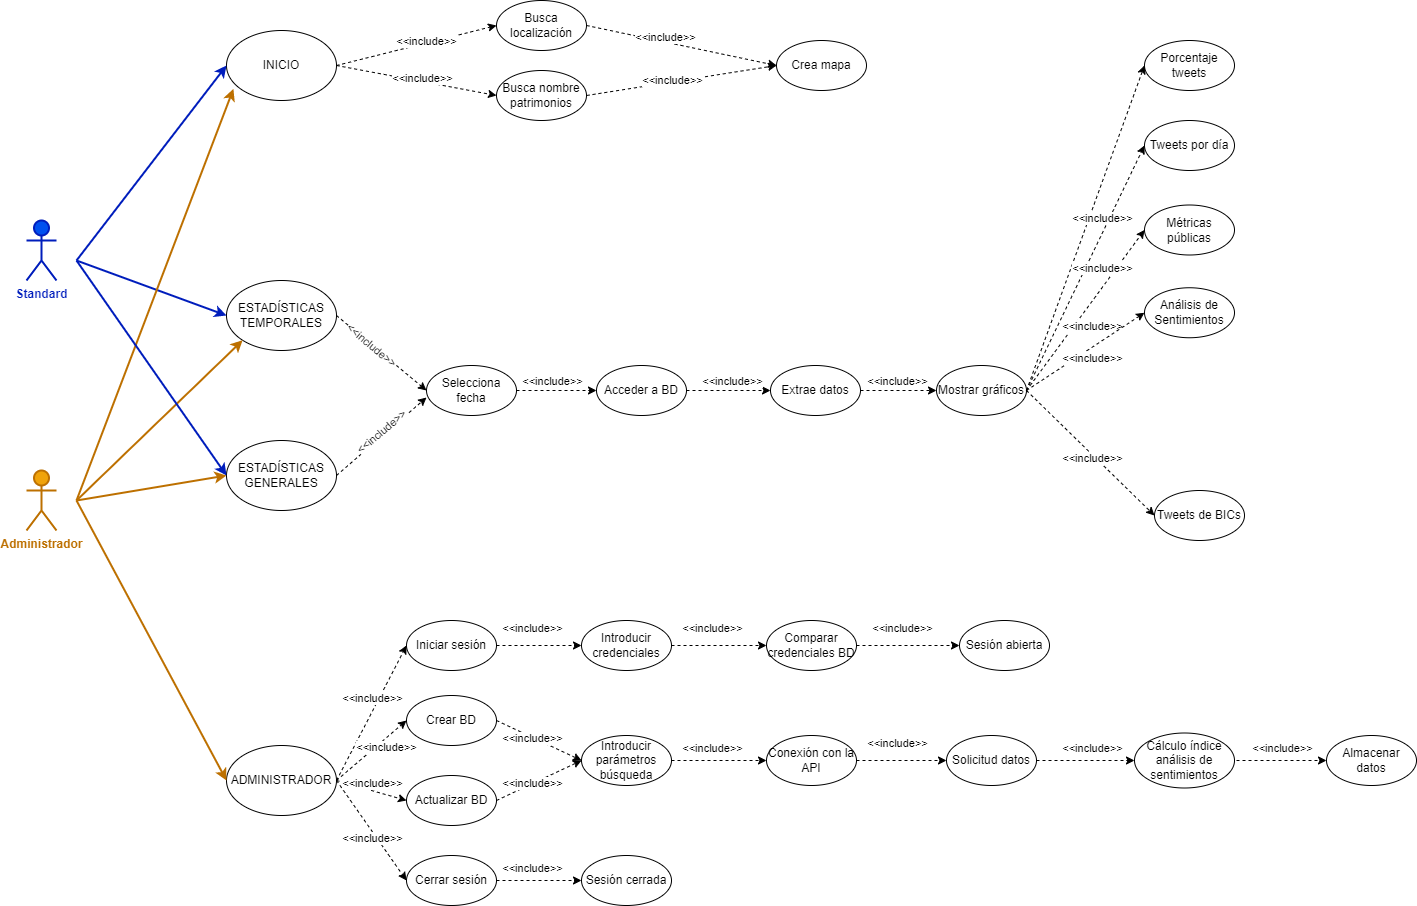
\includegraphics[scale=0.4]{img/casosDeUso.png} \\
        \caption{Especificación de requisitos - Diagrama de caso de uso}
        \label{Especificación de requisitos - Diagrama de caso de uso}
    \end{figure}
\end{landscape}


\subsection{Tablas de caso de uso}
Se muestra a través de tablas, la información de cada requisito del diagrama con sus respectivos parámetros.
% Caso de Uso 1 -> INICIO.
\begin{table}[h!]
	\centering
	\begin{tabularx}{\linewidth}{ p{0.21\columnwidth} p{0.71\columnwidth} }
		\toprule
		\textbf{CU-1}    & \textbf{Inicio}\\
		\toprule
		\textbf{Versión}              & 1.0    \\
		\textbf{Autor}                & Usuario y administrador \\
		\textbf{Requisitos asociados} & RF2, RF3, RF3.1 \\
		\textbf{Descripción}          & Página principal de la aplicación. \\
		\textbf{Precondición}         & Se debe abrir la aplicación en un navegador web. \\
		\textbf{Acciones}             &
		\begin{enumerate}
			\def\labelenumi{\arabic{enumi}.}
			\tightlist
			\item Entrar en el navegador.
			\item Escribir la dirección web.
                \item Si se encuentra en otra página de la aplicación, pulsar en la barra navegadora el boton\textit{'Inicio'}.
		\end{enumerate}\\
		\textbf{Postcondición}        &  -\\
		\textbf{Excepciones}          &  -\\
		\textbf{Importancia}          & Alta \\
		\bottomrule
	\end{tabularx}
	\caption{CU-1 Inicio}
\end{table}
% Caso de Uso 1.1 -> BUSCA LOCALIZACIÓN.
\begin{table}[h!]
	\centering
	\begin{tabularx}{\linewidth}{ p{0.21\columnwidth} p{0.71\columnwidth} }
		\toprule
		\textbf{CU-1.1}    & \textbf{Busca localización}\\
		\toprule
		\textbf{Versión}              & 1.0    \\
		\textbf{Autor}                & Usuario y administrador \\
		\textbf{Requisitos asociados} & RF2, RF3, RF3.1 \\
		\textbf{Descripción}          & Busqueda de localización \\
		\textbf{Precondición}         & Estar en el \textit{'Inicio'}. \\
		\textbf{Acciones}             &
		\begin{enumerate}
			\def\labelenumi{\arabic{enumi}.}
			\tightlist
                \item El programa busca en el csv \textit{inventario\_01} la localización de cada patrimonio.
		\end{enumerate}\\
		\textbf{Postcondición}        &  -\\
		\textbf{Excepciones}          &  -\\
		\textbf{Importancia}          & Baja \\
		\bottomrule
	\end{tabularx}
	\caption{CU-1.1 Busca localización}
\end{table}
% Caso de Uso 1.2 -> BUSCA NOMBRES PATRIMONIOS.
\begin{table}[h!]
	\centering
	\begin{tabularx}{\linewidth}{ p{0.21\columnwidth} p{0.71\columnwidth} }
		\toprule
		\textbf{CU-1.2}    & \textbf{Busca nombre patrimonios}\\
		\toprule
		\textbf{Versión}              & 1.0    \\
		\textbf{Autor}                & Usuario y administrador \\
		\textbf{Requisitos asociados} & RF2, RF3, RF3.1 \\
		\textbf{Descripción}          & Busqueda de nombres de patrimonios \\
		\textbf{Precondición}         & Estar en el \textit{'Inicio'}. \\
		\textbf{Acciones}             &
		\begin{enumerate}
			\def\labelenumi{\arabic{enumi}.}
			\tightlist
                \item El programa busca en el csv \textit{inventario\_01} los nombres de cada patrimonio.
		\end{enumerate}\\
		\textbf{Postcondición}        &  -\\
		\textbf{Excepciones}          &  -\\
		\textbf{Importancia}          & Baja \\
		\bottomrule
	\end{tabularx}
	\caption{CU-1.2 Busca nombre patrimonios}
\end{table}
% Caso de Uso 1.2.1 -> CREAR MAPA.
\begin{table}[h!]
	\centering
	\begin{tabularx}{\linewidth}{ p{0.21\columnwidth} p{0.71\columnwidth} }
		\toprule
		\textbf{CU-1.2.1}    & \textbf{Crear mapa}\\
		\toprule
		\textbf{Versión}              & 1.0    \\
		\textbf{Autor}                & Usuario y administrador \\
		\textbf{Requisitos asociados} & RF2, RF2.1, RF3, RF3.1 \\
		\textbf{Descripción}          & Mapa dinámico con los patrimonios históricos geolocalizados. \\
		\textbf{Precondición}         & Entrar en la página inicio. \\
		\textbf{Acciones}             &
		\begin{enumerate}
			\def\labelenumi{\arabic{enumi}.}
			\tightlist
			\item Entrar en la página \textit{'Inicio'}
			\item Mover con el ratón el mapa
		\end{enumerate}\\
		\textbf{Postcondición}        &  -\\
		\textbf{Excepciones}          &  -\\
		\textbf{Importancia}          & Media \\
		\bottomrule
	\end{tabularx}
	\caption{CU-1.1 Visualización de mapa.}
\end{table}
% Caso de Uso 1.2 -> ELECCION DE PATRIMONIO HISTÓRICO.
\begin{table}[h!]
	\centering
	\begin{tabularx}{\linewidth}{ p{0.21\columnwidth} p{0.71\columnwidth} }
		\toprule
		\textbf{CU-1.2}    & \textbf{Elección de patrimonio histórico}\\
		\toprule
		\textbf{Versión}              & 1.0    \\
		\textbf{Autor}                & Usuario y administrador \\
		\textbf{Requisitos asociados} & RF2, RF2.1, RF2.2 RF3, RF3.1\\
		\textbf{Descripción}          & Elección del patrimonio histórico sobre el mapa. \\
		\textbf{Precondición}         & Entrar en la página inicio. \\
		\textbf{Acciones}             &
		\begin{enumerate}
			\def\labelenumi{\arabic{enumi}.}
			\tightlist
			\item Entrar La página \textit{'Inicio'}
			\item Buscar con el rotón, en el mapa, el patrimonio deseado.
            \item Hacer click sobre él
		\end{enumerate}\\
		\textbf{Postcondición}        &  Hacer click sobre el \textit{'pop up'}\\
		\textbf{Excepciones}          &  Solo se ubican los BICs del Camino de Santiago en la etapa de Castilla y León.\\
		\textbf{Importancia}          & Media \\
		\bottomrule
	\end{tabularx}
	\caption{CU-1.2 Elección de patrimonio histórico.}
\end{table}

% Caso de Uso 2 -> ESTADÍSTICAS TEMPORALES.
\begin{table}[h!]
	\centering
	\begin{tabularx}{\linewidth}{ p{0.21\columnwidth} p{0.71\columnwidth} }
		\toprule
		\textbf{CU-2}    & \textbf{Estadísticas temporales}\\
		\toprule
		\textbf{Versión}              & 1.0    \\
		\textbf{Autor}                & Usuario y administrador \\
		\textbf{Requisitos asociados} & RF1, RF2, RF2.1, RF2.2, RF3, RF3.1\\
		\textbf{Descripción}          & Ventana de la aplicación que contiene todos los gráficos estadísticos sobre el BIC elegido anteriormente, pudiendo cambiar de periodo temporal.  \\
        \textbf{Precondición}         & 
        \begin{enumerate}
			\def\labelenumi{\arabic{enumi}.}
			\tightlist
			\item Entrar en la página \textit{'Inicio'}
			\item Buscar con el ratón, en el mapa, el BIC deseado.
            \item Hacer click sobre él
            \item Hacer click sobre el link incluido en el \textit{pop up'} 
            
		\end{enumerate}\\
		
		\textbf{Acciones}             &
		\begin{enumerate}
			\def\labelenumi{\arabic{enumi}.}
			\tightlist
			\item Visualizar las gráficas.
                \item Selección de fecha.
            
            \item Si se quiere regresar a la página de \textit{'Inicio'}, pulsar sobre el botón de \textit{'Volver'}

		\end{enumerate}\\
		\textbf{Postcondición}        &  Dar al botón \textit{'Volver'}\\
		\textbf{Excepciones}  &
            \begin{enumerate}
                \item La fecha de inicio debe ser anterior a la final.
                \item La base de datos no puede estar vacía.
            \end{enumerate}  \\
            
		\textbf{Importancia}          & Alta \\
		\bottomrule
	\end{tabularx}
	\caption{CU-2 Estadísticas temporales}
\end{table}
% Caso de Uso 3 -> ESTADÍSTICAS GENERALES.
\begin{table}[h!]
	\centering
	\begin{tabularx}{\linewidth}{ p{0.21\columnwidth} p{0.71\columnwidth} }
		\toprule
		\textbf{CU-3}    & \textbf{Estadísticas generales}\\
		\toprule
		\textbf{Versión}              & 1.0    \\
		\textbf{Autor}                & Usuario y administrador \\
		\textbf{Requisitos asociados} & RF1, RF1.6, RF2, RF2.1, RF2.2, RF3, RF3.1, RF3.3\\
		\textbf{Descripción}          & Ventana de la aplicación que contiene el gráfico estadístico comparando todos los BICs, pudiendo cambiar de periodo temporal.  \\
        \textbf{Precondición}         & 
        \begin{enumerate}
			\def\labelenumi{\arabic{enumi}.}
			\tightlist
			\item Entrar en la página \textit{'Inicio'}
			\item En la barra navegadora pulsar sobre \textit{'Estadísticas generales'}.
            
		\end{enumerate}\\
		
		\textbf{Acciones}             &
		\begin{enumerate}
			\def\labelenumi{\arabic{enumi}.}
			\tightlist
			\item Visualizar la gráfica.
                \item Selección de fecha.
            
            \item Si se quiere regresar a la página de \textit{'Inicio'}, pulsar sobre el botón de \textit{'Volver'}

		\end{enumerate}\\
		\textbf{Postcondición}        &  Dar al botón \textit{'Volver'}\\
		\textbf{Excepciones}  &
            \begin{enumerate}
                \item La fecha de inicio debe ser anterior a la final.
                \item La base de datos no puede estar vacía.
            \end{enumerate}  \\
            
		\textbf{Importancia}          & Alta \\
		\bottomrule
	\end{tabularx}
	\caption{CU-3 Estadísticas generales}
\end{table}
% Caso de Uso 2.1 -> SELECCIONA FECHA.
\begin{table}[h!]
	\centering
	\begin{tabularx}{\linewidth}{ p{0.21\columnwidth} p{0.71\columnwidth} }
		\toprule
		\textbf{CU-2.1/3.1}    & \textbf{Selecciona fecha}\\
		\toprule
		\textbf{Versión}              & 1.0    \\
		\textbf{Autor}                & Usuario y administrador \\
		\textbf{Requisitos asociados} & RF1, RF1.4, RF2, RF2.1, RF2.2, RF3, RF3.1\\
		\textbf{Descripción}          & Cambio de fechas para realizar los gráficos temporales.  \\
        \textbf{Precondición}         & 
        \begin{enumerate}
			\def\labelenumi{\arabic{enumi}.}
			\tightlist
			\item Entrar en la página \textit{'Inicio'}
			\item Buscar con el ratón, en el mapa, el BIC deseado.
            \item Hacer click sobre él
            \item Hacer click sobre el link incluido en el \textit{'pop up'} 
            
		\end{enumerate}\\
		
		\textbf{Acciones}             &
		\begin{enumerate}
			\def\labelenumi{\arabic{enumi}.}
			\tightlist
			\item Seleccionar la fecha de inicio en el primer \textit{'input'} que aparece en la parte superior.
                \item Seleccionar la fecha de inicio en el primer \textit{'input'} que aparece en la parte superior.

		\end{enumerate}\\
		\textbf{Postcondición}        &  Dar al botón \textit{'Buscar'} \\
		\textbf{Excepciones}          &  La fecha de inicio debe ser anterior a la final.\\
		\textbf{Importancia}          & Media \\
		\bottomrule
	\end{tabularx}
	\caption{CU-2.1/3.1 Selecciona fecha}
\end{table}
% Caso de Uso 2.1.1 -> ACCEDER A BASE DE DATOS.
\begin{table}[h!]
	\centering
	\begin{tabularx}{\linewidth}{ p{0.21\columnwidth} p{0.71\columnwidth} }
		\toprule
		\textbf{CU-2.1.1/3.1.1}    & \textbf{Acceder a base de datos}\\
		\toprule
		\textbf{Versión}              & 1.0    \\
		\textbf{Autor}                & Usuario y administrador \\
		\textbf{Requisitos asociados} & RF1, RF1.4, RF2, RF2.1, RF2.2, RF3, RF3.1\\
		\textbf{Descripción}          & Se realiza la conexión con la base de datos para realizar operaciones  \\
        \textbf{Precondición}         & 
        \begin{enumerate}
			\def\labelenumi{\arabic{enumi}.}
			\tightlist
			\item Entrar en la página \textit{'Inicio'}
			\item Buscar con el ratón, en el mapa, el BIC deseado.
            \item Hacer click sobre él
            \item Hacer click sobre el link incluido en el \textit{'pop up'} 
            \item Si el usuario ya se encuentra en la página de estadísticas, para realizar la conexión con la base de datos antes se debe pulsar al botón \textit{'buscar'}.
            
		\end{enumerate}\\
		
		\textbf{Acciones}             &
		\begin{enumerate}
			\def\labelenumi{\arabic{enumi}.}
			\tightlist
			\item De manera interna se realiza la conexión con la base de datos mediante psycopg2
            
		\end{enumerate}\\
		\textbf{Postcondición}        &  - \\
		\textbf{Excepciones}          &  La fecha de inicio debe ser anterior a la final.\\
		\textbf{Importancia}          & Alta \\
		\bottomrule
	\end{tabularx}
	\caption{CU-2.1.1/3.1.1 Acceder a base de datos}
\end{table}

% Caso de Uso 2.1.1.1 -> EXTRAE DATOS.
\begin{table}[h!]
	\centering
	\begin{tabularx}{\linewidth}{ p{0.21\columnwidth} p{0.71\columnwidth} }
		\toprule
		\textbf{CU-2.1.1.1/3.1.1.1}    & \textbf{Extrae datos}\\
		\toprule
		\textbf{Versión}              & 1.0    \\
		\textbf{Autor}                & Usuario y administrador \\
		\textbf{Requisitos asociados} & RF1, RF1.4, RF2, RF2.1, RF2.2, RF3, RF3.1\\
		\textbf{Descripción}          & Se realiza la búsqueda de la información requerida del BIC.  \\
        \textbf{Precondición}         & 
        \begin{enumerate}
			\def\labelenumi{\arabic{enumi}.}
			\tightlist
                \item Seleccionar un BIC.
                \item Seleccionar fechas. 
			\item Tener una conexión con la base de datos.
            
		\end{enumerate}\\
		
		\textbf{Acciones}             &
		\begin{enumerate}
			\def\labelenumi{\arabic{enumi}.}
			\tightlist
			\item Se realizan las búsquedas en la base de datos filtrando por el nombre del BIC y las fechas.
            
		\end{enumerate}\\
		\textbf{Postcondición}        &  - \\
		\textbf{Excepciones}          &  La fecha de inicio debe ser anterior a la final.\\
		\textbf{Importancia}          & Alta \\
		\bottomrule
	\end{tabularx}
	\caption{CU-2.1.1.1/3.1.1.1 Extrae datos}
\end{table}

% Caso de Uso 2.1.1.1.1 -> MOSTRAR GRÁFICOS.
\begin{table}[h!]
	\centering
	\begin{tabularx}{\linewidth}{ p{0.21\columnwidth} p{0.71\columnwidth} }
		\toprule
		\textbf{CU-2.1.1.1.1/3.1.1.1.1}    & \textbf{Mostrar gráficos}\\
		\toprule
		\textbf{Versión}              & 1.0    \\
		\textbf{Autor}                & Usuario y administrador \\
		\textbf{Requisitos asociados} & RF1, RF1.1, RF1.2, RF1.3, RF1.4, RF2, RF2.1, RF2.2, RF3, RF3.1\\
		\textbf{Descripción}          & Se realizan los gráficos con la información obtenida de la base de datos.  \\
        \textbf{Precondición}         & 
        \begin{enumerate}
			\def\labelenumi{\arabic{enumi}.}
			\tightlist
                \item Seleccionar un BIC.
                \item Seleccionar fechas. 
			\item Tener una conexión con la base de datos.
                \item Haber obtenido la información que se ha solicitado.
            
		\end{enumerate}\\
		
		\textbf{Acciones}             &
		\begin{enumerate}
			\def\labelenumi{\arabic{enumi}.}
			\tightlist
			\item Realizar los gráficos según los parámetros establecidos.
            
		\end{enumerate}\\
		\textbf{Postcondición}        &  - \\
		\textbf{Excepciones}          &  La fecha de inicio debe ser anterior a la final.\\
		\textbf{Importancia}          & Alta \\
		\bottomrule
	\end{tabularx}
	\caption{CU-2.1.1.1.1/3.1.1.1.1 Mostrar gráficos}
\end{table}

% Caso de Uso 2.1.1.1.1.1 -> PORCENTAJE DE TWEETS.
\begin{table}[h!]
	\centering
	\begin{tabularx}{\linewidth}{ p{0.21\columnwidth} p{0.71\columnwidth} }
		\toprule
		\textbf{CU-2.1.1.1.1.1}    & \textbf{Porcentaje de tweets}\\
		\toprule
		\textbf{Versión}              & 1.0    \\
		\textbf{Autor}                & Usuario y administrador \\
		\textbf{Requisitos asociados} & RF1, RF1.2, RF1.4, RF2, RF2.1, RF2.2, RF3, RF3.1\\
		\textbf{Descripción}          & Se realiza el gráfico de porcentaje de tweets.  \\
        \textbf{Precondición}         & 
        \begin{enumerate}
			\def\labelenumi{\arabic{enumi}.}
			\tightlist
                \item Seleccionar un BIC.
                \item Seleccionar fechas. 
			\item Tener una conexión con la base de datos.
                \item Haber obtenido la información que se ha solicitado.
            
		\end{enumerate}\\
		
		\textbf{Acciones}             &
		\begin{enumerate}
			\def\labelenumi{\arabic{enumi}.}
			\tightlist
			\item Mostrar el gráfico circular con el porcentaje de tweets del BIC en las fechas seleccionadas respecto al total de datos almacenados en la base de datos de todos los patrimonios.
            
		\end{enumerate}\\
		\textbf{Postcondición}        &  - \\
		\textbf{Excepciones}          &  La fecha de inicio debe ser anterior a la final.\\
		\textbf{Importancia}          & Alta \\
		\bottomrule
	\end{tabularx}
	\caption{CU-2.1.1.1.1.1 Porcentaje de tweets}
\end{table}

% Caso de Uso 2.1.1.1.1.2 -> TWEETS POR DIA.
\begin{table}[h!]
	\centering
	\begin{tabularx}{\linewidth}{ p{0.21\columnwidth} p{0.71\columnwidth} }
		\toprule
		\textbf{CU-2.1.1.1.1.2}    & \textbf{Tweets por día}\\
		\toprule
		\textbf{Versión}              & 1.0    \\
		\textbf{Autor}                & Usuario y administrador \\
		\textbf{Requisitos asociados} & RF1, RF1.1, RF1.4, RF2, RF2.1, RF2.2, RF3, RF3.1\\
		\textbf{Descripción}          & Se realiza el gráfico mostrando los tweets generados por día entre las fechas seleccionadas.  \\
        \textbf{Precondición}         & 
        \begin{enumerate}
			\def\labelenumi{\arabic{enumi}.}
			\tightlist
                \item Seleccionar un BIC.
                \item Seleccionar fechas. 
			\item Tener una conexión con la base de datos.
                \item Haber obtenido la información que se ha solicitado.
            
		\end{enumerate}\\
		
		\textbf{Acciones}             &
		\begin{enumerate}
			\def\labelenumi{\arabic{enumi}.}
			\tightlist
			\item Mostrar el gráfico temporal con el número de tweets del BIC en las fechas seleccionadas almacenado en la base de datos.
            
		\end{enumerate}\\
		\textbf{Postcondición}        &  - \\
		\textbf{Excepciones}          &  La fecha de inicio debe ser anterior a la final.\\
		\textbf{Importancia}          & Alta \\
		\bottomrule
	\end{tabularx}
	\caption{CU-2.1.1.1.1.2 Tweets por día}
\end{table}

% Caso de Uso 2.1.1.1.1.3 -> METRICAS PÚBLICAS
\begin{table}[h!]
	\centering
	\begin{tabularx}{\linewidth}{ p{0.21\columnwidth} p{0.71\columnwidth} }
		\toprule
		\textbf{CU-2.1.1.1.1.3}    & \textbf{Métricas públicas}\\
		\toprule
		\textbf{Versión}              & 1.0    \\
		\textbf{Autor}                & Usuario y administrador \\
		\textbf{Requisitos asociados} & RF1, RF1.3, RF1.4, RF2, RF2.1, RF2.2, RF3, RF3.1\\
		\textbf{Descripción}          & Se realiza el gráfico de barras mostrando las métricas públicas del total de tweets al día entre el periodo de tiempo seleccionado.  \\
        \textbf{Precondición}         & 
        \begin{enumerate}
			\def\labelenumi{\arabic{enumi}.}
			\tightlist
                \item Seleccionar un BIC.
                \item Seleccionar fechas. 
			\item Tener una conexión con la base de datos.
                \item Haber obtenido la información que se ha solicitado.
            
		\end{enumerate}\\
		
		\textbf{Acciones}             &
		\begin{enumerate}
			\def\labelenumi{\arabic{enumi}.}
			\tightlist
			\item Mostrar el gráfico temporal apilado con el número de retweets, replies y likes de los tweets de cada uno de los días en el periodo de tiempo seleccionado.
            
		\end{enumerate}\\
		\textbf{Postcondición}        &  - \\
		\textbf{Excepciones}          &  La fecha de inicio debe ser anterior a la final.\\
		\textbf{Importancia}          & Alta \\
		\bottomrule
	\end{tabularx}
	\caption{CU-2.1.1.1.1.3 Métricas públicas}
\end{table}
% Caso de Uso 2.1.1.1.1.4 -> ANÁLISIS DE SENTIMIENTOS
\begin{table}[h!]
	\centering
	\begin{tabularx}{\linewidth}{ p{0.21\columnwidth} p{0.71\columnwidth} }
		\toprule
		\textbf{CU-2.1.1.1.1.4}    & \textbf{Análisis de sentimientos}\\
		\toprule
		\textbf{Versión}              & 1.0    \\
		\textbf{Autor}                & Usuario y administrador \\
		\textbf{Requisitos asociados} & RF1, RF1.3, RF1.4, RF1.5, RF2, RF2.1, RF2.2, RF3, RF3.1\\
		\textbf{Descripción}          & Se realiza el gráfico semicircular mostrando el valor del análisis de sentimientos de los tweets del BIC seleccionado entre las fechas elegidas.  \\
        \textbf{Precondición}         & 
        \begin{enumerate}
			\def\labelenumi{\arabic{enumi}.}
			\tightlist
                \item Seleccionar un BIC.
                \item Seleccionar fechas. 
			\item Tener una conexión con la base de datos.
                \item Haber obtenido la información que se ha solicitado.
            
		\end{enumerate}\\
		
		\textbf{Acciones}             &
		\begin{enumerate}
			\def\labelenumi{\arabic{enumi}.}
			\tightlist
			\item Realizar la media de los valores del análisis de sentimientos de todos los tweets del BIc entre las fechas seleccionadas.
                \item Mostrar con un gráfico semicircular el valor numérico del análisis de sentimientos.
            
		\end{enumerate}\\
		\textbf{Postcondición}        &  - \\
		\textbf{Excepciones}          &  La fecha de inicio debe ser anterior a la final.\\
		\textbf{Importancia}          & Alta \\
		\bottomrule
	\end{tabularx}
	\caption{CU-2.1.1.1.1.4 Análisis de sentimientos}
\end{table}

% Caso de Uso 3.1.1.1.1.1 -> TWEETS de BICs
\begin{table}[h!]
	\centering
	\begin{tabularx}{\linewidth}{ p{0.21\columnwidth} p{0.71\columnwidth} }
		\toprule
		\textbf{CU-3.1.1.1.1.1}    & \textbf{Tweets de BICs}\\
		\toprule
		\textbf{Versión}              & 1.0    \\
		\textbf{Autor}                & Usuario y administrador \\
		\textbf{Requisitos asociados} & RF1, RF1.2, RF1.4, RF1.6 RF2, RF2.1, RF2.2, RF3, RF3.1, RF3.3\\
		\textbf{Descripción}          & Se realiza el gráfico de total de tweets de los BICs.  \\
        \textbf{Precondición}         & 
        \begin{enumerate}
			\def\labelenumi{\arabic{enumi}.}
			\tightlist
                \item Pulsar en la barra navegadora el botón 'Estadístias generales'.
                \item Seleccionar fechas. 
			\item Tener una conexión con la base de datos.
            
		\end{enumerate}\\
		
		\textbf{Acciones}             &
		\begin{enumerate}
			\def\labelenumi{\arabic{enumi}.}
			\tightlist
			\item Mostrar el gráfico con la comparación de los tweets publicados de todos los BICs entre las fechas seleccionadas.
            
		\end{enumerate}\\
		\textbf{Postcondición}        &  - \\
		\textbf{Excepciones}          &  La fecha de inicio debe ser anterior a la final.\\
		\textbf{Importancia}          & Alta \\
		\bottomrule
	\end{tabularx}
	\caption{CU-3.1.1.1.1.1 Tweets de BICs}
\end{table}
% Caso de Uso 4 -> ADMINISTRADOR.
\begin{table}[h!]
	\centering
	\begin{tabularx}{\linewidth}{ p{0.21\columnwidth} p{0.71\columnwidth} }
		\toprule
		\textbf{CU-4}    & \textbf{Administrador}\\
		\toprule
		\textbf{Versión}              & 1.0    \\
		\textbf{Autor}                & Administrador \\
		\textbf{Requisitos asociados} & RF3.2, RF3.2.1, RF3.2.2, RF3.2.3, RF4.2.4, RF4, RF5, RF5.1, RF5.1.1, RF5.1.2, RF5.1.3, RF5.1.4, RF5.2, RF5.2.1, RF5.2.2, RF5.2.3, RF5.3\\
		\textbf{Descripción}          & Ventana de la aplicación que contiene la acción \textit{'Iniciar sesión'} desde la que se podrán realizar las acciones del rol administrador  \\
        \textbf{Precondición}         & Abrir la aplicación \\
		\textbf{Acciones}             &
		\begin{enumerate}
			\def\labelenumi{\arabic{enumi}.}
			\tightlist
			\item Entrar en la página \textit{'Inicio'}
			\item En la barra navegadora hacer click sobre \textit{'Administrador'} para ver las opciones que se sugieren
		\end{enumerate}\\
		\textbf{Postcondición}     &   
        \begin{enumerate}
			\def\labelenumi{\arabic{enumi}.}
			\tightlist
			\item Hacer \textit{'Iniciar sesión'}
			\item Pulsar una de las opciones del desplegable. 
		\end{enumerate}\\
		\textbf{Excepciones}          & -\\
		\textbf{Importancia}          & Media \\
		\bottomrule
	\end{tabularx}
	\caption{CU-4 Administrador.}
\end{table}




% Caso de Uso 4.1 -> INICIAR SESIÓN
\begin{table}[h!]
	\centering
	\begin{tabularx}{\linewidth}{ p{0.21\columnwidth} p{0.71\columnwidth} }
		\toprule
		\textbf{CU-4.1}    & \textbf{Iniciar sesión}\\
		\toprule
		\textbf{Versión}              & 1.0    \\
		\textbf{Autor}                & Administrador \\
		\textbf{Requisitos asociados} & RF3.2, RF3.2.1, RF4, RF5, RF5.1, RF5.1.1, RF5.1.2, RF5.1.3, RF5.1.4, RF5.2, RF5.2.1, RF5.2.2, RF5.2.3, RF5.3\\
		\textbf{Descripción}          & Permite ver la ventana que posibilita al usuario ingresar con unas credenciales para acceder indentificándose como administrador\\
        \textbf{Precondición}         &  
  		\begin{enumerate}
			\def\labelenumi{\arabic{enumi}.}
			\tightlist
			\item Entrar en la página \textit{'Inicio'}
			\item En la barra navegadora hacer click sobre \textit{'Iniciar sesión'}
		\end{enumerate}\\
		\textbf{Acciones}             &
		\begin{enumerate}
			\def\labelenumi{\arabic{enumi}.}
			\tightlist
			\item Ver pestaña de \textit{'Inicio de sesión'}.
		\end{enumerate}\\
		\textbf{Postcondición}     &   Insertar credenciales \\
		\textbf{Excepciones}          & - \\
		\textbf{Importancia}          & Alta \\
		\bottomrule
	\end{tabularx}
	\caption{CU-4.1 Iniciar sesión}
\end{table}

% Caso de Uso 4.1.1 -> INTRODUCIR CREDENCIALES
\begin{table}[h!]
	\centering
	\begin{tabularx}{\linewidth}{ p{0.21\columnwidth} p{0.71\columnwidth} }
		\toprule
		\textbf{CU-4.1.1}    & \textbf{Introducir credenciales}\\
		\toprule
		\textbf{Versión}              & 1.0    \\
		\textbf{Autor}                & Administrador \\
		\textbf{Requisitos asociados} & RF5, RF5.1, RF5.1.1, RF5.1.2, RF5.1.3, RF5.1.4, RF5.2, RF5.2.1, RF5.2.2, RF5.2.3, RF5.3\\
		\textbf{Descripción}          & Permite al usuario ingresar con unas credenciales para entrar como administrador\\
        \textbf{Precondición}         &  
  		\begin{enumerate}
			\def\labelenumi{\arabic{enumi}.}
			\tightlist
			\item Entrar en la página \textit{'Inicio'}
			\item En la barra navegadora hacer click sobre \textit{'Iniciar sesión'}
		\end{enumerate}\\
		\textbf{Acciones}             &
		\begin{enumerate}
			\def\labelenumi{\arabic{enumi}.}
			\tightlist
			\item Insertar usuario.
                \item Insertar contraseña.
		\end{enumerate}\\
		\textbf{Postcondición}     &   Comprobar credenciales \\
		\textbf{Excepciones}          & - \\
		\textbf{Importancia}          & Alta \\
		\bottomrule
	\end{tabularx}
	\caption{CU-4.1.1 Introducir credenciales}
\end{table}

% Caso de Uso 4.1.1.1 -> COMPARAR CREDENCIALES
\begin{table}[h!]
	\centering
	\begin{tabularx}{\linewidth}{ p{0.21\columnwidth} p{0.71\columnwidth} }
		\toprule
		\textbf{CU-4.1.1.1}    & \textbf{Comparar credenciales}\\
		\toprule
		\textbf{Versión}              & 1.0    \\
		\textbf{Autor}                & Administrador \\
		\textbf{Requisitos asociados} & RF5, RF5.1, RF5.1.1, RF5.1.2, RF5.1.3, RF5.1.4, RF5.2, RF5.2.1, RF5.2.2, RF5.2.3, RF5.3\\
		\textbf{Descripción}          & Permite comprobar si el usuario es administrador o no.\\
        \textbf{Precondición}         &  
  		\begin{enumerate}
			\def\labelenumi{\arabic{enumi}.}
			\tightlist
			\item Entrar en la página \textit{'Inicio'}
			\item En la barra navegadora hacer click sobre \textit{'Iniciar sesión'}
                \item Insertar usuario.
                \item Insertar contraseña.
		\end{enumerate}\\
		\textbf{Acciones}             &
		\begin{enumerate}
			\def\labelenumi{\arabic{enumi}.}
			\tightlist
			\item Buscar en la base de datos en la tabla \textit{'Usuarios'} el nombre de usuario introducido.
   			\item Si el nombre se encuentra en la base de datos, se comprueba si la contraseña introducida es la misma que la contraseña encriptada de la base de datos.
		\end{enumerate}\\
		\textbf{Postcondición}     &   Abrir la sesión \\
		\textbf{Excepciones}          & - \\
		\textbf{Importancia}          & Alta \\
		\bottomrule
	\end{tabularx}
	\caption{CU-4.1.1.1 Comparar credenciales}
\end{table}

% Caso de Uso 4.1.1.1.1 -> SESION ABIERTA
\begin{table}[h!]
	\centering
	\begin{tabularx}{\linewidth}{ p{0.21\columnwidth} p{0.71\columnwidth} }
		\toprule
		\textbf{CU-4.1.1.1.1}    & \textbf{Sesión abierta}\\
		\toprule
		\textbf{Versión}              & 1.0    \\
		\textbf{Autor}                & Administrador \\
		\textbf{Requisitos asociados} & RF5, RF5.1, RF5.1.1, RF5.1.2, RF5.1.3, RF5.1.4, RF5.2, RF5.2.1, RF5.2.2, RF5.2.3, RF5.3\\
		\textbf{Descripción}          & Marcar al usuario como administrador\\
        \textbf{Precondición}         &  
  		\begin{enumerate}
			\def\labelenumi{\arabic{enumi}.}
			\tightlist
			\item Entrar en la página \textit{'Inicio'}.
			\item En la barra navegadora hacer click sobre \textit{'Iniciar sesión'}.
                \item Insertar usuario.
                \item Insertar contraseña.
                \item Comprobar credenciales.
		\end{enumerate}\\
		\textbf{Acciones}             &
		\begin{enumerate}
			\def\labelenumi{\arabic{enumi}.}
			\tightlist
			\item Introducir 'True' el parámetro 'identificado' de la sesión para que la aplicación sepa que tienes los permisos de administrador.
   			
		\end{enumerate}\\
		\textbf{Postcondición}     &  Seleccionar opciones de administrador. \\
		\textbf{Excepciones}          & - \\
		\textbf{Importancia}          & Media \\
		\bottomrule
	\end{tabularx}
	\caption{CU-4.1.1.1.1 Sesión abierta}
\end{table}

% Caso de Uso 4.2 -> CREAR BASE DE DATOS
\begin{table}[h!]
	\centering
	\begin{tabularx}{\linewidth}{ p{0.21\columnwidth} p{0.71\columnwidth} }
		\toprule
		\textbf{CU-4.2}    & \textbf{Crear base de datos}\\
		\toprule
		\textbf{Versión}              & 1.0    \\
		\textbf{Autor}                & Administrador \\
		\textbf{Requisitos asociados} & RF5, RF5.1, RF5.1.1, RF5.1.2, RF5.1.3, RF5.1.4, RF5.2, RF5.2.1, RF5.2.2, RF5.2.3, RF5.3\\
		\textbf{Descripción}          & Permite al usuario crear una base de datos desde una fecha inicio hasta una fecha fin.\\
        \textbf{Precondición}         &  
  	\begin{enumerate}
			\def\labelenumi{\arabic{enumi}.}
			\tightlist
			\item Entrar en la página. \textit{'Inicio'}.
			\item En la barra navegadora hacer click sobre \textit{'Iniciar sesión'}.
            \item Ingresar usuario y contraseña.

		\end{enumerate}\\
		\textbf{Acciones}             &
		\begin{enumerate}
			\def\labelenumi{\arabic{enumi}.}
			\tightlist
			\item Pulsar sobre \textit{'Crear base de datos'}
            \item Insertar los parámetros que se requieren:            
            \begin{enumerate}
    			\def\labelenumi{\arabic{enumi}.}
    			\tightlist
    			\item Número de peticiones totales por cada periodo de tiempo de espera especificado.
                \item El tiempo de espera para el total de peticiones especificado.
                \item El tiempo de espera de cada una de las peticiones.
		  \end{enumerate}
            \item El programa se conectará con la API de Twitter y obtendrá la información requerida.
            \item El programa se encargará de introducir en la base de datos la información en cada una de las columnas.
		\end{enumerate}\\
		\textbf{Postcondición}     &   Esperar a la carga completa de datos.\\
		\textbf{Excepciones}          & 
        \begin{enumerate}
            \def\labelenumi{\arabic{enumi}.}
            \tightlist
            \item Salir de la página de carga de datos mientras se está ejecutando.
            \item Pedir más peticiones de las permitidas por la API de Twitter en un periodo de tiempo.
            \item Introducir menor tiempo de espera para el número total de peticiones admitidas del permitido por la API de Twitter.
            \item Introducir menor tiempo de espera para cada petición del permitido por la API de Twitter.
            \item Ejecutar el proceso de carga de datos simultáneamente en otro equipo.
            \item Realizar dos operaciones de administrador seguidas en el tiempo.
		\end{enumerate}\\
		\textbf{Importancia}          & Alta \\
		\bottomrule
	\end{tabularx}
	\caption{CU-4.2 Crear base de datos}
\end{table}

% Caso de Uso 4.3 -> ACTUALIZAR BASE DE DATOS
\begin{table}[h!]
	\centering
	\begin{tabularx}{\linewidth}{ p{0.21\columnwidth} p{0.71\columnwidth} }
		\toprule
		\textbf{CU-4.3}    & \textbf{Actualizar base de datos}\\
		\toprule
		\textbf{Versión}              & 1.0    \\
		\textbf{Autor}                & Administrador \\
		\textbf{Requisitos asociados} & FR3.2.3,RF5, RF5.2, RF5.2.1, RF5.2.2, RF5.3, RF5.3\\
		\textbf{Descripción}          & Permite al usuario actualizar la base de datos, desde la última fecha registrada en la base de datos hasta la fecha actual.\\
        \textbf{Precondición}         &  
  	\begin{enumerate}
			\def\labelenumi{\arabic{enumi}.}
			\tightlist
			\item Entrar en la página \textit{'Inicio'}.
			\item En la barra navegadora hacer click sobre \textit{'Iniciar sesión'}.
            \item Ingresar usuario y contraseña.
		\end{enumerate}\\
		\textbf{Acciones}             &
		\begin{enumerate}
			\def\labelenumi{\arabic{enumi}.}
			\tightlist
			\item Pulsar sobre \textit{'Actualizar base de datos'}.
            \item Insertar los parámetros que se requieren:
            \begin{enumerate}
    			\def\labelenumi{\arabic{enumi}.}
    			\tightlist
    			\item Número de peticiones totales por cada periodo de tiempo de espera especificado.
                \item El tiempo de espera para el total de peticiones especificado.
                \item El tiempo de espera de cada una de las peticiones.
		  \end{enumerate}
            \item El programa se conectará con la API de Twitter y obtendrá la información requerida.
            \item El programa se encargará de introducir en la base de datos la información en cada una de las columnas.
		\end{enumerate}\\
		\textbf{Postcondición}     &   Esperar a la carga completa de datos. \\
		\textbf{Excepciones}          & 
        \begin{enumerate}
            \def\labelenumi{\arabic{enumi}.}
            \tightlist
            \item Salir de la página de carga de datos mientras se está ejecutando.
            \item Pedir más peticiones de las permitidas por la API de Twitter en un periodo de tiempo.
            \item Introducir menor tiempo de espera para el número total de peticiones admitidas del permitido por la API de Twitter.
            \item Introducir menor tiempo de espera para cada petición del permitido por la API de Twitter.
            \item Ejecutar el proceso de carga de datos simultáneamente en otro equipo.
            \item Realizar dos operaciones de administrador seguidas en el tiempo.
		\end{enumerate}\\
		\textbf{Importancia}          & Alta \\
		\bottomrule
	\end{tabularx}
	\caption{CU-4.3 Actualizar base de datos}
\end{table}

% Caso de Uso 4.2.1/4.3.1 -> INTRODUCIR PARÁMETROS DE BÚSQUEDA
\begin{table}[h!]
	\centering
	\begin{tabularx}{\linewidth}{ p{0.21\columnwidth} p{0.71\columnwidth} }
		\toprule
		\textbf{CU-4.2.1/4.3.1}    & \textbf{Introducir parámetros de búsqueda}\\
		\toprule
		\textbf{Versión}              & 1.0    \\
		\textbf{Autor}                & Administrador \\
		\textbf{Requisitos asociados} & FR3.2.3,RF5, RF5.2, RF5.2.1, RF5.2.2, RF5.3, RF5.3\\
		\textbf{Descripción}          & Insertar los parámetros necesarios para realizar la búsqueda en la API de Twitter.\\
        \textbf{Precondición}         &  
  	\begin{enumerate}
			\def\labelenumi{\arabic{enumi}.}
			\tightlist
			\item Entrar en la página \textit{'Inicio'}.
			\item En la barra navegadora hacer click sobre \textit{'Iniciar sesión'}.
            \item Ingresar usuario y contraseña.
		\end{enumerate}\\
		\textbf{Acciones}             &
		\begin{enumerate}
			\def\labelenumi{\arabic{enumi}.}
			\tightlist
			\item Pulsar sobre \textit{'Actualizar base de datos'}.
            \item Insertar los parámetros que se requieren:
            \begin{enumerate}
    			\def\labelenumi{\arabic{enumi}.}
    			\tightlist
    			\item Número de peticiones totales por cada periodo de tiempo de espera especificado.
                \item El tiempo de espera para el total de peticiones especificado.
                \item El tiempo de espera de cada una de las peticiones.
		  \end{enumerate}
            
		\end{enumerate}\\
		\textbf{Postcondición}     &   Pulsar sobre el botón buscar. \\
		\textbf{Excepciones}          & 
        \begin{enumerate}
            \def\labelenumi{\arabic{enumi}.}
            \tightlist
            \item Introducir una fecha anterior a 2006.
		\end{enumerate}\\
		\textbf{Importancia}          & Media\\
		\bottomrule
	\end{tabularx}
	\caption{CU-4.2.1/4.3.1 Actualizar base de datos}
\end{table}

% Caso de Uso 4.2.1.1/4.3.1.1 -> CONEXIÓN CON LA API
\begin{table}[h!]
	\centering
	\begin{tabularx}{\linewidth}{ p{0.21\columnwidth} p{0.71\columnwidth} }
		\toprule
		\textbf{CU-4.2.1.1/4.3.1.1}    & \textbf{Conexión con la API}\\
		\toprule
		\textbf{Versión}              & 1.0    \\
		\textbf{Autor}                & Administrador \\
		\textbf{Requisitos asociados} & FR3.2.3,RF5, RF5.2, RF5.2.1, RF5.2.2, RF5.3, RF5.3\\
		\textbf{Descripción}          & Realizar la conexión con la API de Twitter.\\
        \textbf{Precondición}         &  
  	\begin{enumerate}
			\def\labelenumi{\arabic{enumi}.}
			\tightlist
			\item Ser administrador.
            \item Haber introducido los parámetros requeridos.
		\end{enumerate}\\
		\textbf{Acciones}             &
		\begin{enumerate}
			\def\labelenumi{\arabic{enumi}.}
			\tightlist
            \item Pasar los parámetros seleccionados al servicio que realiza la búsqueda.
            \item Realizar la conexión con la API de twitter a través de un \textit{endpoint}.
		  \end{enumerate}\\
            
		\textbf{Postcondición}     &   Extraer datos. \\
		\textbf{Excepciones}          & 
        \begin{enumerate}
            \def\labelenumi{\arabic{enumi}.}
            \tightlist
            \item Introducir parámetros que no admita la API de twitter (más solicitudes de las permitidas, menor tiempo de espera...)
		\end{enumerate}\\
		\textbf{Importancia}          & Alta\\
		\bottomrule
	\end{tabularx}
	\caption{CU-4.2.1.1/4.3.1.1 Conexión con la API}
\end{table}

% Caso de Uso 4.2.1.1.1/4.3.1.1.1 -> SOLICITUD DE DATOS
\begin{table}[h!]
	\centering
	\begin{tabularx}{\linewidth}{ p{0.21\columnwidth} p{0.71\columnwidth} }
		\toprule
		\textbf{CU-4.2.1.1.1/4.3.1.1.1}    & \textbf{Solicitud de datos}\\
		\toprule
		\textbf{Versión}              & 1.0    \\
		\textbf{Autor}                & Administrador \\
		\textbf{Requisitos asociados} & FR3.2.3,RF5, RF5.2, RF5.2.1, RF5.2.2, RF5.3, RF5.3\\
		\textbf{Descripción}          & Pedir los datos que se necesitan a la API de Twitter.\\
        \textbf{Precondición}         &  
  	\begin{enumerate}
			\def\labelenumi{\arabic{enumi}.}
			\tightlist
			\item Ser administrador.
                \item Haber introducido los parámetros requeridos.
                \item Haber realizado la conexión con la API de Twitter.
		\end{enumerate}\\
		\textbf{Acciones}             & Pedir, por cada día de tweets, que te devuelva todos los parámetros especificados.\\
		\textbf{Postcondición}     &   Almacenar datos en base de datos. \\
		\textbf{Excepciones}          & 
        \begin{enumerate}
            \def\labelenumi{\arabic{enumi}.}
            \tightlist
            \item Introducir parámetros que no admita la API de twitter (más solicitudes de las permitidas, menor tiempo de espera...)
		\end{enumerate}\\
		\textbf{Importancia}          & Alta\\
		\bottomrule
	\end{tabularx}
	\caption{CU-4.2.1.1.1/4.3.1.1.1 Solicitud de datos}
\end{table}
% Caso de Uso 4.2.1.1.1.1/4.3.1.1.1.1 -> Cálculo índice análisis de sentimientos
\begin{table}[h!]
	\centering
	\begin{tabularx}{\linewidth}{ p{0.21\columnwidth} p{0.71\columnwidth} }
		\toprule
		\textbf{CU-4.2.1.1.1.1/4.3.1.1.1.1}    & \textbf{Cálculo índice análisis de sentimientos}\\
		\toprule
		\textbf{Versión}              & 1.0    \\
		\textbf{Autor}                & Administrador \\
		\textbf{Requisitos asociados} & RF1.5, RF3.2.3,RF5, RF5.2, RF5.2.1, RF5.2.2, RF5.3, RF5.3\\
		\textbf{Descripción}          & Calcular el índice de sentimiento (positivo o negativo) de cada tweet.\\
        \textbf{Precondición}         &  
  	\begin{enumerate}
			\def\labelenumi{\arabic{enumi}.}
			\tightlist
			\item Ser administrador.
            \item Haber introducido los parámetros requeridos.
		\end{enumerate}\\
		\textbf{Acciones}             &
		\begin{enumerate}
			\def\labelenumi{\arabic{enumi}.}
			\tightlist
            \item Obtener todos los nuevos registros de la base de datos.
            \item Calcular el índice de sentimiento de cada uno de ellos.
            \item Introducir el valor en la columna \textit{'Tweet_SentimentAnalysis'}.
		  \end{enumerate}\\
            
		\textbf{Postcondición}     &   Guardar la transacción \\
		\textbf{Excepciones}          & 
        \begin{enumerate}
            \def\labelenumi{\arabic{enumi}.}
            \tightlist
            \item -
		\end{enumerate}\\
		\textbf{Importancia}          & Alta\\
		\bottomrule
	\end{tabularx}
	\caption{CU-4.2.1.1.1.1/4.3.1.1.1.1 Cálculo índice análisis de sentimientos}
\end{table}
% Caso de Uso 4.2.1.1.1.1.1/4.3.1.1.1.1.1 -> ALMACENAR DATOS
\begin{table}[h!]
	\centering
	\begin{tabularx}{\linewidth}{ p{0.21\columnwidth} p{0.71\columnwidth} }
		\toprule
		\textbf{CU-4.2.1.1.1.1.1/4.3.1.1.1.1.1}    & \textbf{Almacenar datos}\\
		\toprule
		\textbf{Versión}              & 1.0    \\
		\textbf{Autor}                & Administrador \\
		\textbf{Requisitos asociados} & FR3.2.3,RF5, RF5.2, RF5.2.1, RF5.2.2, RF5.3, RF5.3\\
		\textbf{Descripción}          & Almacenar la información recopilada en la base de datos\\
        \textbf{Precondición}         &  
  	\begin{enumerate}
			\def\labelenumi{\arabic{enumi}.}
			\tightlist
			\item Ser administrador
                \item Haber introducido los parámetros requeridos.
                \item Haber realizado la conexión con la API de Twitter
		\end{enumerate}\\
		\textbf{Acciones}             &
		\begin{enumerate}
			\def\labelenumi{\arabic{enumi}.}
			\tightlist
            \item Abrir la conexión con la base de datos.
            \item Repetir por cada día de recopilación, y una vez recopilados todos los días del patrimonio, se continua con el siguiente hasta terminar con todos.
            \item Cerrar conexión con la base de datos.
            \end{enumerate}\\
            
		\textbf{Postcondición}     &   Volver a inicio \\
		\textbf{Excepciones}          & 
        \begin{enumerate}
            \def\labelenumi{\arabic{enumi}.}
            \tightlist
            \item Introducir parámetros que no admita la API de twitter (más solicitudes de las permitidas, menor tiempo de espera...)
		\end{enumerate}\\
		\textbf{Importancia}          & Media\\
		\bottomrule
	\end{tabularx}
	\caption{CU-4.2.1.1.1.1.1/4.3.1.1.1.1.1 Almacenar datos}
\end{table}

% Caso de Uso 4.4 -> CERRAR SESIÓN
\begin{table}[h!]
	\centering
	\begin{tabularx}{\linewidth}{ p{0.21\columnwidth} p{0.71\columnwidth} }
		\toprule
		\textbf{CU-4.4}    & \textbf{Cerrar sesión}\\
		\toprule
		\textbf{Versión}              & 1.0    \\
		\textbf{Autor}                & Administrador \\
		\textbf{Requisitos asociados} & FR3.2.2, RF5.3\\
		\textbf{Descripción}          & El usuario puede cerrar la sesión de rol administrador.\\
        \textbf{Precondición}         &  
  		\begin{enumerate}
			\def\labelenumi{\arabic{enumi}.}
			\tightlist
			\item Entrar en la página \textit{'Inicio'}.
                \item Ser administrador.
		\end{enumerate}\\
		\textbf{Acciones}             &
		\begin{enumerate}
			\def\labelenumi{\arabic{enumi}.}
			\tightlist
			\item En la barra navegadora hacer click sobre \textit{'Cerrar sesión'}.
            \item Si se ha iniciado sesión recientemente, en la pestaña de opciones del administrador pulsar sobre \textit{'Cerrar sesión'}.
            
		\end{enumerate}\\
		\textbf{Postcondición}     &   - \\
		\textbf{Excepciones}          & - \\
		\textbf{Importancia}          & Alta \\
		\bottomrule
	\end{tabularx}
	\caption{CU-4.4 Cerrar sesión}
\end{table}

% Caso de Uso 4.4.1 -> SESION CERRADA
\begin{table}[h!]
	\centering
	\begin{tabularx}{\linewidth}{ p{0.21\columnwidth} p{0.71\columnwidth} }
		\toprule
		\textbf{CU-4.4.1}    & \textbf{Sesión cerrada}\\
		\toprule
		\textbf{Versión}              & 1.0    \\
		\textbf{Autor}                & Administrador \\
		\textbf{Requisitos asociados} & FR3.2.2, RF5.3\\
		\textbf{Descripción}          & El usuario puede cerrar la sesión de rol administrador\\
        \textbf{Precondición}         &  
  		\begin{enumerate}
			\def\labelenumi{\arabic{enumi}.}
			\tightlist
			\item Entrar en la página \textit{'Inicio'}.
                \item Ser administrador.
		\end{enumerate}\\
		\textbf{Acciones}             &
		\begin{enumerate}
			\def\labelenumi{\arabic{enumi}.}
			\tightlist
			\item En la barra navegadora hacer click sobre \textit{'Cerrar sesión'}.
            \item Si se ha iniciado sesión recientemente, en la pestaña de opciones del administrador, pulsar sobre \textit{'Cerrar sesión'}.
            \item Insertar 'False' en el parámetro 'identificado' de la sesión, para que el programa pueda detectar que el usuario no tiene permisos de administrador.
		\end{enumerate}\\
		\textbf{Postcondición}     &   - \\
		\textbf{Excepciones}          &  - \\
		\textbf{Importancia}          & Alta \\
		\bottomrule
	\end{tabularx}
	\caption{CU-4.4.1 Sesión cerrada}
\end{table}
 